Online forums generally have a specific structure that provides a lot of
context to all the interactions occuring among the users. Ignoring this in the
analysis makes researhers lose a lot of precious information as we will see in
later sections.
Here we describe a typeical forum \& related structure and the answers that we
are looking for.

\subsection{Structure in online forums}
In an online forum when two users interact in a thread or through a post
they probably bring from their own individual point of views or come
form possibly different communities.
It is valuable to know which topic/community they each belong to in that
interaction. When a user U is representing community C out of all communties
that he is part of, he tailors his post content accordingly to suit the
explicit or implicit community norms. Knowing the style of community
specific text content provides a lot of information about the community in general. 
It also provides information about what role user U plays when he is in community
C. In online forums multi-user interactions happen a lot i.e.
in a thread a user can post by addressing to another specific user but he is
also addressing other users in the thread explicitly or implicitly. Modeling
this phenomenon would bring our model closer to reality. This knowledge 
can be modelled by aggregating
users posts acorss a thread, though not across the whole of the forum. We will
elaborate on this more in the generative story section.
Another interesting property of such structured conversations is that there is 
an inherent bias towards the thread starter or in turn topic of the thread. 
It would be interesting to see what 
insights this knowledge provides given that a model can make use of such an
information (\comment{This would be very relevant for post-and-response
forums in our dataset such as Reddit and Stack Overflow. Right now our graphical
model doesn't support this but it would be interesting to see how this can be brought in. It might not be too difficult to do this}).


\subsection{Graphical model \& generative story}
Based on the discussions above our graphical model is designed as shown
in figure~\ref{fig:finalThreadAggregationModel}. In this model,
figure~\ref{fig:finalThreadAggregationModel} below, we aggregate the posts of 
a given user in a given thread into one document called $R_p$. This helps us
incorporate the knowledge that a user's post is influenced by all the posts of
other users present on the thread.

The generative process for the model is as follows:

\begin{figure}
\centering
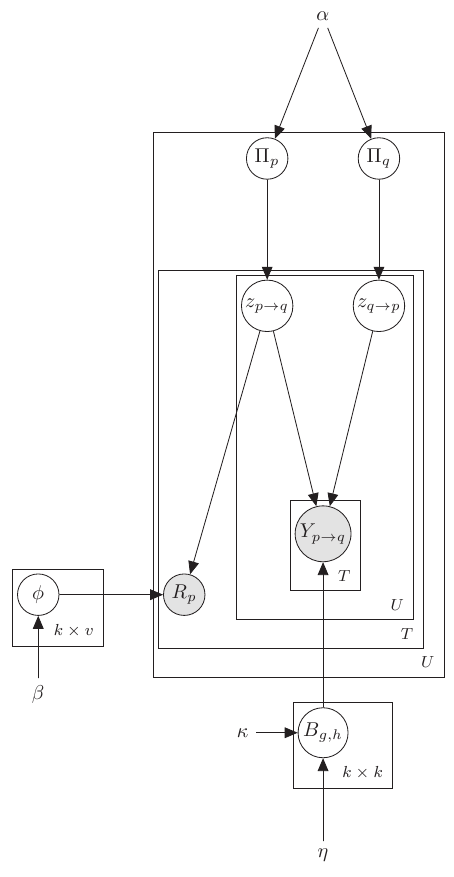
\includegraphics[width=0.6\textwidth]{pgm_ThreadBased.png}
\caption{This graphical model takes into account multi-way interaction among
users in a thread simultaneously}
\label{fig:finalThreadAggregationModel}
\end{figure}

Assuming that there are total $N_t$ users in the thread $t$.  
\begin{itemize}
  \item For each Thread $t$
\begin{itemize}
  \item For each user $p \in \mathcal{N}_t$
  \begin{itemize}
    \item Draw a $K$ dimensional mixed membership vector 
    $\overset{\rightarrow}{\uppi}_{p} \sim$ Dirichlet($\alpha$)

    \item Draw $B(g,h) \sim Gamma(\kappa,\eta)$; where $\kappa, \eta$ are
    parameters of the gamma distribution.
  \end{itemize}

  \item For each pair of users $(p, q) \in \mathcal{N}_t \times \mathcal{N}_t$:
  \begin{itemize}
    \item Draw membership indicator for the indicator, 
    $\overset{\rightarrow}{z}_{(p \rightarrow q,t)} \sim$
    Multinomial($\uppi_{p}$).
    \item Draw membership indicator for the receiver,
    $\overset{\rightarrow}{z}_{(q \rightarrow p,t)} \sim$
    Multinomial($\uppi_{q}$).
    \item Sample the value of their interaction, $Y(p,q,t) \sim$
    Poisson(${\overset{\rightarrow}{z}}^{\top}_{(p \rightarrow q,t)}
    B~\overset{\rightarrow}{z}_{(p \leftarrow q,t)}$). 
	\end{itemize}
	\item For each user $p \in \mathcal{N}_t$
	\begin{itemize}
	  \item Draw $\phi_{k}$ from $Dirichlet(\beta)$.
	  \item Form the set $Q_{p,t}$ that contains all the users that p interacts to
	  on thread $t$
	  \begin{itemize}
	    \item For each word $w \in R_{p,t}$ 
	    \item Draw $w \sim \phi(w|z_{(p \rightarrow q,t)}, \forall q\in Q_{p,t})$  
	  \end{itemize}
  \end{itemize}
\end{itemize}  
\end{itemize}

The data likelihood for the model in figure~1

\begin{eqnarray}
P(Y, R_{p} | \alpha, \beta, \kappa, \eta) = \int_{\Phi} \! \int_{\Pi} \sum_{z} \! P(Y, R_{p}, z_{p \rightarrow q}, z_{p \leftarrow q}, \Phi, \Pi | 
\alpha, \beta, \kappa, \eta)  \nonumber \\  \nonumber
\\ = \int_{\Phi} \! \int_{\Pi} \sum_{z} \! \bigg[ \prod_{p,q} \prod_{t}
P(Y_{pq}^{t} | z_{p \rightarrow q}^{t}, z_{p \leftarrow q}^{t}, B) 
\cdot P(z_{p \rightarrow q}^{t} | \Pi_{p}) \cdot P(z_{p \leftarrow q}^{t} |
\Pi_{q})  \nonumber
\\ \cdot \left(\prod_{p} P(\Pi_{p} | \alpha) \prod_{t} \prod_{p} P(R_{p}^{t} |
z_{p \rightarrow q}^{t}, \Phi) \cdot \prod_{k} P(\Phi_{k} | \beta)\right) \cdot
\prod_{g,h}P(B_{gh} | \eta, \kappa) \bigg]
\end{eqnarray}

The complete log likeliood of the model is:

\begin{align}
\log \! P(Y, W, z_{\rightarrow}, z_{\leftarrow}, \Phi, \Pi, B | \kappa, \eta,
\beta, \alpha) = \sum_{t} \! \sum_{p,q} \! \log P(Y_{pq}^{t} | z_{p \rightarrow
q}^{t} , z_{p \leftarrow q}^{t}, B)~+ \nonumber  \\\nonumber \sum_{t} \!
\sum_{p,q} \! (\log P(z_{p \rightarrow q}^{t} | \Pi_{p}) + \log \! P(z_{p \leftarrow q}^{t} |
\Pi_{p})) + \sum_{p} \! \log \! P(\Pi_{p} | \alpha) ~+\\  \sum_{t} \!
\sum_{p} \! \sum_{w \in R_{p}^{t}} \log P(w | z_{p \rightarrow}, \Phi) +
\sum_{k} \! \log P(\Phi_{k} | \beta) + \sum_{gh} \! \log P(B_{gh} | \eta,
\kappa)
\end{align}

The mean field variational approximation for the posterior is 

\begin{align}
q(z, \Phi, \Pi, B | \Delta_{z_{\rightarrow}}, \Delta_{\Phi}, \Delta_{B},
\Delta_{z_{\leftarrow}}, \Delta_{B_{\kappa}}) = \prod_{t} \! \prod_{p,q} \!
\bigg( q_{1}(z_{p \rightarrow q}^{t} | \Delta_{z_{p \rightarrow q}}) +
q_{1}(z_{p \leftarrow q}^{t} | \Delta_{z_{p \leftarrow q}})  \bigg) \nonumber \\
\cdot \prod_{p} \! q_{4}(\Pi_{p} | \Delta_{\Pi_{p}}) \prod_{k} q_{3} (\Phi_{k} |
\Delta_{\Phi_{k}}) \prod_{g,h} \! q(B_{g,h} | \Delta_{B_{\eta}}, \Delta_{B_{\kappa}})
\end{align}

The lower bound for the data log-likelihood from jensen's inequality is: 

\begin{align}
L_{\Delta} &= E_{q}\bigg[ \log \! P(Y, W, z_{\rightarrow}, z_{\leftarrow}, \Phi,
\Pi, B | \kappa, \eta, \beta, \alpha) - \log \! q \bigg]
\end{align}

\begin{eqnarray}
L_{\Delta} = E_{q} \Bigg[ \sum_{t} \! \sum_{p,q} \! \log \left(
B_{g,h}^{Y_{p,q}^t} \frac{e^{-B_{gh}}}{Y_{pq}^{t}!} \right) +
\sum_{t} \! \sum_{pq} \! \log\left( \prod_{k} (\pi_{p,k}^{z_{p \rightarrow q} =
k}) \right) + \sum_{t} \! \sum_{p,q} \log \! \left( \prod_{k}(\pi_{q,k})^{z_{p
\leftarrow q} = k} \right) ~+ \nonumber\\
 \sum_{p} \! \log \left( \prod_{k}
(\Pi_{p,k})^{\alpha_{k} - 1} \cdot \frac{\Gamma(\sum \alpha_{k})}{\prod_{k}
\Gamma(\alpha_{k})} \right) +
\sum_{t} \! \sum_{p} \! \sum_{w\in R_p^t}  \log \! \left(
\prod_{u\in V}(\bar{z}^T\phi_u)^{w = u} \right) + \nonumber\\
 \sum_{k} \! \log\left( \prod_{u\in V}
(\phi_{k,u})^{\beta_{k} - 1} \cdot \frac{\Gamma(\sum \beta_{k})}{\prod_{k}
\Gamma(\beta_{k})} \right) +
 \sum_{g,h} \! \log \! \left( B_{g,h}^{\kappa - 1} /
\eta^{\kappa} \Gamma(\kappa) \cdot \exp(-B_{g,h}/\eta) \right) \Bigg]
\nonumber\\
% 
% \end{eqnarray}
% \begin{eqnarray}
 -E_{q} \Bigg[ \sum_{t} \! \sum_{p,q} \log \big( \prod_{k} (\Delta_{z_{p
\rightarrow q}, k})^{z_{p \rightarrow q}=k} \big) + \sum_{t} \! \sum_{p,q}
\! \log \! \left(
\prod_{k} \! (\Delta_{z_{p \leftarrow q}, k})^{z_{p \leftarrow q} = k} \right)
 + \nonumber \\
 \sum \! \log \left( \prod_{k} \! (\Pi_{p,k})^{\Delta_{\pi_{pk}}-1}
\frac{\Gamma(\Delta_{\Pi_{p}})}{\prod_{k=1} \! \Gamma(\Delta_{\Pi_{p,k}})}
\right) + 
\sum_{k} \log \! \left( \prod_{u \in v}
(\Phi_{k,u})^{\Delta_{\Phi_{ku}} - 1)} \frac{\Gamma(\Delta_{\Phi_{k}})}
{\prod_{u \in v} \! \Gamma(\Delta_{\Phi_{k,u}})} \right) + \nonumber \\ 
\sum_{g,h} \log \! \left(
\frac{B_{g,h}^{\Delta_{\kappa = 1}}}{\Delta_{\eta}^{\Delta_{\kappa}}
\Gamma(\Delta_{\kappa})} \exp(-B_{g,h}/\Delta_{\eta}) \right) \Bigg]
\label{eqn:VarLowerBound}
\end{eqnarray}


Equation~\ref{eqn:VarLowerBound} is the variational lower bound of the log
likelihood function which is to be maximized.
There are terms like $ E_q\left[\sum_{g,h} \! \log \! \left( B_{g,h}^{\kappa -
1} / \eta^{\kappa} \Gamma(\kappa) \cdot \exp(-B_{g,h}/\eta) \right) \right]$
which can be obtained by taking derivation of the partition function of the exponential
family form of gamma distribution. An effective way
to evaluate $E_q\left[ \sum_{t} \! \sum_{p} \! \sum_{w\in R_p^t}  \log \! \left(
\prod_{u\in V}(\bar{z}^T\phi_u)^{w = u} \right)\right]$ 
is by introducing an additional latent variable $\bar{z}_p$ which is a
realization of the average $\frac{\sum_{q\in Q} z_{p\rightarrow q}}{|Q|}$. 
~\comment{So figure~\ref{fig:finalThreadAggregationModel} will be modifed
slightly in future where $R_p$ is drawn from $\bar{z}$ and $\bar{Z}$ is drawn from
$z_{p\rightarrow q}$. This was suggested by Chong as well as Eric but I
finally figured out the equation of the vriational approximation for this. I
will update the equations once I have coded it and verified.}.
